\documentclass[12pt, a4paper, twoside]{article}

\usepackage[CJKchecksingle]{xeCJK}
\usepackage{fontspec}
\usepackage{adjustbox}
\usepackage{graphicx}
\usepackage{wrapfig}
\usepackage{xcolor}
\usepackage{listings}

\setCJKmainfont{WenQuanYi Micro Hei}
\setCJKmonofont{WenQuanYi Micro Hei Mono}
\setromanfont{Droid Serif}
\setmonofont{Droid Sans Mono}
\parindent 2em

\renewcommand{\abstractname}{摘要}
\renewcommand{\figurename}{圖}
\renewcommand{\tablename}{表}
\pagestyle{headings}

\begin{document}
\title{探索Xelatex:使用中文維基百科的Firefox條目}
\author{佐倉祈\thanks{製作Xelatex原始碼(格式化)}
  \and 維基百科Firefox條目貢獻者\thanks{內文真正的作者!請感謝他們!}}
\date{\today}
\maketitle

\begin{abstract}
這是一份測試文件。文件的內容是複製自Wikipedia的Firefox條目。總之文字什
麼的都不重要,請看版面吧!
\end{abstract}

Mozilla Firefox,中文俗稱為“火狐”(被中国官方使用但未注册為商標),是由
Mozilla基金會採用開放原始碼與社群共同開發的網頁瀏覽器。可以在多種作業系
統執行,原始碼以GPL/LGPL/MPL三種授權方式釋出。\footnote{好複雜的授權}

2012年8月,Firefox在全球網頁瀏覽器市場上占約23\%,為第三大廣泛使用的網
頁瀏覽器。在各國家、地區之中,印度尼西亚、德國和波蘭為Firefox佔有率最高
的國家及地區,各佔77.2\%、57.17\% 和51.68\% 的使用率。

\section{發展歷程}
Mozilla Firefox最初是由戴夫·海厄特、喬伊·休伊斯及布雷克·羅斯建立的實驗
性分支。他們認為网景公司資助的商業需求及開發者導向的功能膨脹會降低瀏覽
器的易用性[11],因此從功能複雜的Mozilla Application Suite中分支出獨立的
瀏覽器。

該專案的名称經過多次波折,最初稱作Phoenix,但因為和鳳凰科技(Phoenix
  Technologies)的名稱衝突,于是改為Firebird。後來,这个新名称又与另一
個開放原始碼的資料庫系統Firebird发生了冲突,Firebird的開發社群要求以全
稱Mozilla Firebird來标识這個專案或重新命名,避免混淆。\footnote{原來有
  這樣的典故!}

2004年2月9日,Mozilla Firebird決定改稱Mozilla Firefox,簡稱Firefox,正
式縮寫為Fx或fx[12],不過仍然常被稱作FF(FireFox)。雖然Firefox在英文俗
語裡指的是小熊貓(学名:Ailurus fulgens)[13],但是開發小組卻是使用直譯
的方法,因此吉祥物及官方圖示的設計都是火紅的小狐狸,因此為了避免與動物
小熊貓的「Firefox」混淆,官方採用全稱「Mozilla Firefox」。

\section{特色}

Firefox包含了許多突出的特色,像是分頁瀏覽、拼字檢查、遞增搜尋、即時書籤、
下載管理員、自訂搜尋引擎、私密瀏覽…等等。Firefox的開發目標是「盡情的上
  網瀏覽」和「對多數人來說最棒的上網體驗」[14]。

使用者可以透過附加元件和佈景主題(Theme)來自定义Firefox的功能和外觀,
在Mozilla維護的附加元件網站中,已經有36,861種的附加元件可供下載(包括實
  驗中元件有10,720種)[15](截至2010年6月20日為止)。

對於網頁開發者,Firefox也提供一個良好的開發平台。網頁開發者可以透過內建
的工具來進行開發工作,例如:錯誤主控台、DOM觀察器,此外還可透過附加元件
像是Firebug、Web Developer來延伸開發功能。

\subsection{支援多種網路標準}

% It's not recommended to have footnotes in captions of figure/table
\begin{figure}
\centering
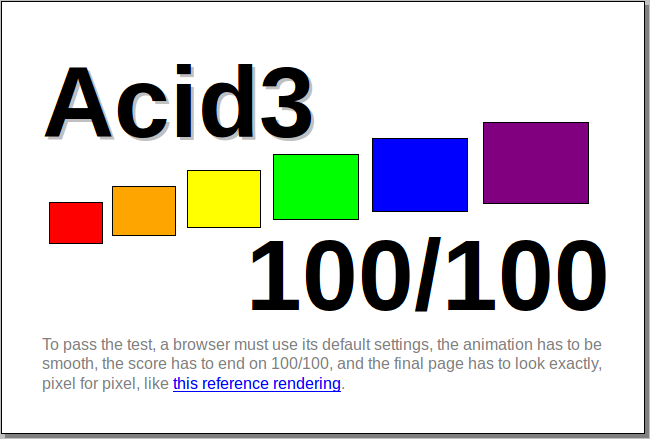
\includegraphics[width=70mm]{Firefox_7_Acid_3_Result}
\caption{Firefox 7在Acid3\protect\footnotemark測試的結果
  \protect\footnotemark}
\end{figure}
\addtocounter{footnote}{-2}
\stepcounter{footnote}
\footnotetext{Acid3??}
\stepcounter{footnote}
\footnotetext{現在19已經出了唷!}

Firefox支援非常多的網路標準,包含了HTML、XML、XHTML、SVG 1.1(部份的)、
CSS(除了標準之外,還有擴充的支援[16])、ECMAScript(JavaScript)、DOM、
MathML、DTD、XSLT、XPath和PNG圖檔(包含透明度支援)[17]。

雖然Firefox 2並沒有通過Acid2網路標準測試,不過在Firefox 3.0 Alpha 2時通
過Acid2測試和Acid3 71/100項測試, Firefox 3.1的版本可通過Acid3 93/100項
測試,Firefox 3.6達到Acid3 94/100的標準,到Firefox 7.0版本更已達到
Acid3 100/100滿分標準 [18]。

\subsection{安全性}

Firefox使用了「沙盒安全模組」(Sandbox Security Model)[19],限制了網頁
腳本語言對使用者端資料的存取,保護使用者不受惡意腳本語言的攻擊。對於網
頁資料的傳輸,則使用SSL/TLS的加密方式來保障使用者和網站之間傳輸資料的隱
密性[20],此外也支援智慧卡來當作資料驗證的方式[21]。

從Firefox 2.0起Mozilla就與Google一起合作,為使用者提供反釣魚保護,當
Firefox 2.0在遇到釣魚網站後使用者可馬上得到提示。Firefox的黑名單來自於
Google搜尋中的SafeBrowsing Protocol[22][23],而從2009年的1月20日起
Google正式關閉Firefox 2.0的反釣魚技術,[24][25] 但是對Firefox 3及最新版
本依然提供保護。

自Firefox 4開始,Mozilla新增了「內容安全政策」(Content Security
  Policy),其中包含了對於跨網站指令碼(XSS)攻擊的防禦措施。

Mozilla基金會提供了「臭蟲獎金」來獎勵發現Firefox及旗下產品漏洞的研究者
[26],獎金為3000美元[27],為軟體產業最早提出臭蟲獎勵制度的公司。
Mozilla官方希望安全弱點可以在被惡意利用之前被發現,進而去修正他,避免使
用者遭受攻擊[28]。

因為Firefox比起Internet Explorer來說有較少尚未修正的安全漏洞(參見網頁
  瀏覽器比較),因此提昇上網安全性也常常被認為是鼓勵使用者由Internet
Explorer轉換到Firefox的理由之一[29][30][31][32]。《華盛頓郵報》也報導在
2006年一年之中,Internet Explorer共有284天讓使用者暴露在未修正的安全漏
洞中,而Firefox只有9天[33]。

一份2006年賽門鐵克(Symantec)公司的報告顯示,到該年9月為止,雖然
Firefox的安全漏洞比其他瀏覽器多,但修正漏洞的速度讓其他瀏覽器望塵莫及
[34]。但在經過安全性的研究後澄清了之前的描述,Firefox比起Internet
Explorer來說安全漏洞還是比較少[35]。到2008年3月26日為止, 根據軟體安全
統計網站Secunia的資料顯示,Firefox 2有4個尚未修正的安全漏洞,多數被標示
為「低度危險」[36]。相對的Internet Explorer 7卻有8個安全漏洞尚未修正,
且多數被標示為「中度危險」[37]。甚至有安全專家建議微軟IE升級模式效仿
Firefox瀏覽器,如果在現行版本中發現重大安全漏洞,就應即時釋出漏洞更新
[38]。

2011年12月\marginpar{這段展示了陰謀論},Accuvant安全測試公司在由Google
資助的一項研究的研究報告中指出,Internet Explorer 9安全性已相當接近同期
的Google Chrome 15,反觀同期的Mozilla Firefox 9則居於其後[39],但隨後有
NSS Labs安全測試公司指此項研究有失中立性,並指出Accuvant公司曾接受
Google的巨額贊助,在研究過程中Firefox的許多安全特性也被刻意忽略而未作測
試,選取測試用惡意外掛模組的方式亦有偏袒Chrome打壓Firefox之嫌[40]。

2012年中旬,Mozilla在Firefox 14中引入了''click to play(點選播放)''這
一新的安全機制。[41]這一安全機制預設情況下不會啟用,但一旦使用者啟用了
這一安全機制之後,Firefox將不會自動顯示或播放在網頁上的第三方外掛模組內
容,比如Flash動畫,而是會顯示一個對話方塊讓使用者選擇是否顯示或播放外掛
模組內容。這種外掛模組提醒功能除了提升瀏覽器的安全性防止攻擊者利用某些
外掛模組中的漏洞之外,也同時防止了很多過期的外掛模組導致瀏覽器崩潰的情
況。[42]而在2013年一月Mozilla在其部落格中吐露,未來所釋出的Firefox中或
將遮蔽掉除了最新版本的 Adobe Flash 之外的其他所有外掛模組,像Java、
Adobe Reader和微軟的Silverlight外掛模組。若使用者使用,則需要手動載入。
[43]

\subsection{智慧位址列}

在Firefox瀏覽器的網址列中輸入文字時會顯示符合的書籤和歷史。增加可設定的
搜尋符號時(與搜尋關鍵字中間要有空格),會顯示限定的搜尋結果,規則如下:

\begin{adjustbox}{center}
\footnotesize\linespread{1.2}\centering\begin{tabular}{lll} \hline
about:config &  預設的搜尋符號 & 顯示結果\\ \hline
browser.urlbar.match.title & \# & 顯示與網頁標題符合的結果\\
browser.urlbar.match.url & @ & 顯示與網頁位址符合的結果\\
browser.urlbar.restrict.bookmark & * & 只顯示書籤中的結果\\
browser.urlbar.restrict.history & \^{} & 只顯示歷史記錄中的結果\\
browser.urlbar.restrict.tag & + & 只顯示增加了分頁的結果\\
browser.urlbar.restrict.typed & \~{} & 只顯示在網址列輸入過的字元\\
browser.urlbar.restrict.openpage & \% & 只顯示開啟的分頁\\ \hline
\end{tabular}
\end{adjustbox}

\subsection{附加元件}

擴充套件、佈景主題、外掛程式的總稱。可以從Mozilla官方維護的 附加元件官
方網站 下載,或是從其他的第三方開發者取得。

\subsection{擴充套件}

Firefox使用者可以透過安裝擴充套件來新增或修改Firefox的功能
\marginpar[(左文)如右,這裡說明了Firefox最棒的功能]{(右文)如左,這
  裡說明了Firefox最棒的功能}。擴充套件的種類包羅萬象:像滑鼠手勢、廣告
視窗阻擋、加強的分頁瀏覽等等。擴充套件雖然提供了高度自由化的擴充功能,
但是使用者可能在尋找和安裝擴充套件上遭遇困難,也會建議把擴充套件的功能
整合到Firefox中,像是分頁瀏覽就是從一個Mozilla上的附加元件MultiZilla中
移植過來的。[44]

多數的擴充套件不是由Mozilla建立或支援的,擴充套件在使用者的電腦中也具有
存取資料的權限,因此也有出現過惡意的擴充套件[45]。甚至有些病毒專門利用
某些擴充套件來盜取使用者的網路銀行密碼。[46] Mozilla提供了對擴充套件的
驗證,來確保這些志願開發者提供的附加元件沒有包含任何惡意軟體。此外由第
三方開發者所製作的擴充套件,Mozilla並不保證可以在Mozilla的產品上運作,
也可能包含任何軟體錯誤或者安全漏洞[47]。

\subsection{即時尋找}

Firefox提供加強的搜尋功能,包含了快速的「隨打即找」功能,使用者只需要在
尋找框輸入要尋找的字串,按F3後就可以自動標示出要尋找的字串。
\subsection{即時書籤}

透過即時書籤,使用者可以以書籤的方式來閱讀RSS或Atom訂閱項目,這個功能第
一次出現在Firefox 1.0的預覽版,隨後也移植到了Mozilla Suite中。即時書籤
會自動更新,也可以在右鍵選單中手動選擇更新。即時標題

若網站提供 即時摘要(網頁中定期更新之關鍵訊息的摘要),使用者的書籤標題
便能更換為此「即時標題」。隨時更新、比起固定的網頁標題更能提供有用訊息,
恰好適合做為書籤的標題。已經有 許多網站 能以即時標題的方式加入書籤,還
有 其他附加元件 能幫您建立某些熱門網站的即時標題。

\subsection{文字選取}

Firefox瀏覽器提供了便捷的文字選取操作,在網頁文字上滑鼠左鍵雙擊可以選取
一個詞,三擊可以選取一段話。按住Ctrl鍵(蘋果機上是Cmd鍵)可以在不取消已
選取文字的前提下選取其它文字。

\subsection{在地化}

Firefox是一個非常注重在地化的網頁瀏覽器。自2004年11月正式發布的初始版本
起,即提供包括28種不同的語言版本,包括正體中文、簡體中文、美國英語、英
國英語以及歐洲西班牙語、阿根廷西班牙語版本,至今已達到86種語言版本。管
理網路存取許可權

Firefox使用者能自訂存取某些網站的許可權。在網址列輸入
「about:\allowbreak{}permissions」開啟就會進入Firefox的許可權管理器頁面,
該頁面中會顯示使用者存取過的站點,並記錄這些網站的儲存密碼、共享位置訊
息、Cookie設定、開啟彈出窗口、維護離線儲存等許可權的設定,使用者可以根
據自己的需要去設定這些站點可存取的許可權[48]。

\section{推廣活動}

隨著2004年Firefox首次正式發佈開始,就開始展開一系列的推廣活動,而隨著這
些活動,Firefox在一年後就迅速的達到1億次的下載數量[49]。而在2009年的8月
份Firefox的下載量就突破性地達到了10億次。這只是對其官方網站統計而所作出
的結果,而不包括從其他網站下載的次數[50]。

2004年9月12日,簡稱為SFX的「Spread Firefox」網站正式隨著Firefox 1.0預覽
版一起推出[51],網站提供了各種推廣Firefox方式的訊息交換中心。

而「世界Firefox日」活動則是在Firefox的建立者:Mozilla基金會三週年紀念日
2006年8月15日開始,為期兩個月,到2006年9月15日為止。參與活動的人或者網
站有機會在Firefox朋友之牆(Firefox Friends Wall)上留名,這是一個位於
Mozilla基金會總部的數位顯示版[52]。

2004年10月21日,Mozilla基金會號召支持者買下紐約時報全版廣告,刊登即將在
11月釋出的Firefox 1.0。短短十天的募捐活動已經獲得來自一萬人的25萬美元捐
款[53]。

2006年4月27日,Mozilla於舊金山國際電影節舉辦了Firefox Flicks短片比賽,
由來自全世界300多個Firefox愛好者當中選出四支最佳的短片,這些影片會被用
來於波士頓與舊金山地區的電視台放送,幫助推廣Firefox。頭獎為Pete
Macomber製作的Daredevil[54]。

% wrapfigure and figure environment are different
% so here, \addtocounter should be added HERE!
\addtocounter{footnote}{-3}
\begin{wrapfigure}{R}{0.5\textwidth}
  \begin{center}
    
\includegraphics[width=55mm]{Firefox_Crop_Circle}
  \end{center}
  \caption{Firefox麥田圈共動員十二人\protect\footnotemark,籌劃了兩個星
    期,在24小時內製作完成\protect\footnotemark,直徑達220英呎。
    \protect\footnotemark}
\end{wrapfigure}

\addtocounter{footnote}{-3}
\stepcounter{footnote}
\footnotetext{十二人:一打人}

\stepcounter{footnote}
\footnotetext{一打人,兩打小時。可見規劃的重要。}

\stepcounter{footnote}
\footnotetext{我的語無倫次是為了讓這張圖可以擁有三個註腳XD然而,這樣設
  置註腳會造成註腳可能和圖不在同一頁}

2006年8月12日,為慶祝Firefox下載量達2億,美國奧勒岡州立大學Linux小組
Firefox專案(Oregon State University Linux Group Firefox project)在奧
勒岡州附近燕麥田所製作的Firefox麥田圈,出現在Google地圖與Google地球上
[55]。

2008年2月21日,Firefox的下載數量到達了5億次,Firefox的社群發動到網站
FreeRice猜問題,取得5億顆米來慶祝 [56]。

2008年,在Mozilla Firefox 3.0正式發佈前,社群發動Firefox Download
Day(直譯為Firefox下載日),希望重新整理金氏世界紀錄中「單日最多人下載
  軟體」的一項。支持者需預先到推廣網站Spread Firefox登記,在Fx 3.0發佈
當日便會收到電郵提示參與活動[57]。

Firefox3自發佈至6月18日凌晨重新整理24小時下載金氏世界紀錄,並且在48小時
下載超過1200萬(以上數字均不包括自動更新)。

2008年10月,雖然獲得了大量使用者的下載,但是據Mozilla公司的統計資料表示
約有75\%的下載者並不使用Firefox作為他們的瀏覽器[58]。而據CnBeta資訊網站
相關的資料統計,在有移除Firefox的使用者中,有30\%來自中國,排在後面的分
別是美國(23\%),日本、巴西和德國(9\%)[59]。為此Mozilla公司就開始了
一個叫做「Impact Mozilla」的推廣計劃,徵求來自全球各地網友的推廣創意,
如何讓下載了Firefox的使用者們成為真正Mozilla的忠實用戶(見 Impact
  Mozilla首頁)。

而在中國,Mozilla推出了火狐中國版(Mozilla Firefox China Edition)專門
為中國使用者定製。在Firefox 3的基礎上做了很多包括拖曳文字、股市查詢、音
樂收聽在內的在地化工作,使其儘量符合中國使用者的使用習慣(見 火狐中國首
  頁)。

2009年8月5日,Mozilla台灣社群推出抓火狐推廣平台,使用OpenID登入即可打造
專屬你的個人化推廣貼紙(見 抓火狐首頁)。

2009年11月10日,Firefox誕生五週年(見 Firefox五週年慶首頁)。

2010年9月14日,Mozilla推出了一款瀏覽器基準測試工具Kraken(Kraken測試頁
  面),基於SunSpider改良,Mozilla宣稱該測試更符合使用者真實網路使用情
形,雖然Kraken為官方發佈,所得出的測試資料的中立性有待商榷,但Kraken基
於開放原始碼,歡迎更多社群來參與和貢獻 [60][61]。

\section{評價}

網站《Forbes.com》稱Firefox為「2004年最佳瀏覽器」[62],雜誌《PC World》
在「2005年最佳百大產品」中也將Firefox列入[63],在Firefox 2和Internet
Explorer 7推出的2006年,PC World也對這兩個瀏覽器做出評論,並認為
Firefox是比較好的瀏覽器[64]。雜誌《Which?》也提名Firefox為最佳的網頁瀏
覽器。[65] 英國Vnunet網站甚至把Firefox的市場佔有率的不斷攀升列為10大鼓
舞人心IT事件之一。[66]

媒體《Internet Week》在一篇文章中提到許多讀者在使用Firefox 1.5時記憶體
用量相當的高[67]。Mozilla的開發團隊表示Firefox 1.5記憶體用量的升高是因
為新的「上一頁/下一頁」(FastBack)功能所導致的[68]。此外設計錯誤的擴
充套件,像是某些舊版的Adblock[69],或者一些外掛程式(plug-ins)[70] 也
是造成記憶體使用量增多的原因。《PC Magazine》比較了Firefox、Opera、
Internet Explorer這三個瀏覽器的記憶體使用量,認為Firefox的記憶體使用量
接近其他兩個瀏覽器[71]。另外由《PC World》和《Zimbra》的測試也指出
Firefox 2的記憶體用量少於Internet Explorer 7[64][72],還在測試中的
Firefox 3(以beta 1版本來進行測試)記憶體使用量沒有低於Firefox 2,不過
仍然少於Internet Explorer 7。[73]

如同其他的瀏覽器一樣,Firefox也有一些安全漏洞,可能會影響使用者的電腦安
全,不過根據 CERT 的統計,Firefox的安全漏洞也少於Internet Explorer。

《Softpedia》的測試指出Firefox比起其他瀏覽器需要比較長的啟動時間
[74][75],IE 6也比Firefox有稍快的啟動速度,不過這是因為IE用到的程式組件
有些在Windows啟動後就載入了,因此會有較快的啟動時間。

但也有評論家大唱反調,在一篇刊登在《PC World》雜誌上的分析文章稱,在與
Chrome瀏覽器的競爭中,火狐瀏覽器正逐漸失去電腦專家的青睞。儘管Mozilla基
金會仍致力於一些宏大的標的,但火狐瀏覽器已經宣告死亡。\footnote{在我看
  來Firefox依舊充滿了活力。更何況實際上來說,Firefox是自由軟體界最棒的
  瀏覽器}[76]

事實上,Chrome 與 Firefox 並非你死我活的對手。Google 在2011年12月尾便與
Firefox 達成協議,Google 在未來三年將繼續成為Firefox 的預設搜尋引擎。雖
然雙方均沒有透露作價,但市傳金額為約每年3 億美元。[77]

\section{獎項}

Mozilla Firefox自推出之後便得到許多的獎項,包含了:

\begin{itemize}
\item CNET編輯推薦,2011年3月[78]
\item Webware百大軟體,2009年5月[79]
\item PC World 2009最佳免費軟體,2009年1月[80]
\item PC Magazine編輯推薦,2008年6月[81]
\item PC World 2008年度百大產品,2008年5月[82]
\item Webware百大軟體,2008年4月[83]
\item Webware百大軟體,2007年6月[84]
\item PC World 2007年度百大產品,2007年5月[85]
\item PC Magazine編輯推薦,2006年10月[86]
\end{itemize}

\section{市場接納度}

% SVG cannot be used directly
% converted pdf file is used instead.
\begin{wrapfigure}{l}{0.5\textwidth}
  \begin{center}
    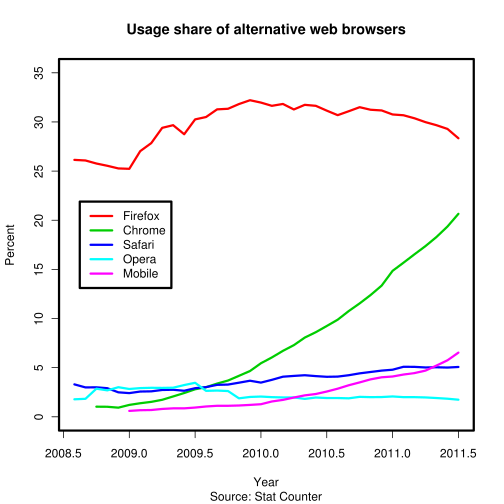
\includegraphics[width=70mm]{Usage}
  \end{center}
  \caption{非IE的瀏覽器市佔率變化。}
\end{wrapfigure}

Mozilla Firefox市佔率從發行初期就開始不斷的增加,大多數是因為Internet
Explorer的市佔率降低而來。自Firefox釋出開始,Internet Explorer的佔有率
便穩定的下降。

Firefox的下載次數自2004年11月釋出1.0後持續的增加,截自2009年7月31日,
Firefox下載次數已突破一億[100]。這是官方的統計數字,並不包含透過軟體更
新或者其他第三方網站的下載數量[101]。而且下載數量並不能反應實際的使用者
數,因為一個使用者可能同時在很多台電腦上下載並安裝。

這樣快速的成長以至於有網路媒體稱Firefox將在2013年超越IE。[102] 但是微軟
卻對這些數字表示質疑。[103] 有媒體甚至具體列舉出了10條Firefox將擊敗微軟
IE的理由。[104] 這也就不奇怪在微軟2008年向美國證券交易委員會送出的10-K
管理檔案中稱,Firefox已對微軟Windows業務構成威脅,這也是微軟首次公開把
Firefox當作Windows業務競爭對手[105]。

2010年7月2日,IBM公司近40萬名的員工將使用預載Firefox瀏覽器的電腦。
[106]

然而,從2012年開始,Firefox的市佔率有所衰退,主因是競爭對手Google
Chrome市佔率的大幅增加。但仍與IE、Chrome保持「三足鼎立」局面。

\section{程式碼測試(不是原始條目的一部分)}
來一段Haskell程式碼!

% Use literate replacement to prevent '--' -> long dash conversion!
\begin{lstlisting}[language=Haskell, extendedchars=true, literate={--}{{\texttt{--}}}{2}]
module Main where
-- 中文註解
main :: IO ()
main = putStrLn "Hello, World!"
\end{lstlisting}

另外來一段C程式碼!

% modified from wikibook
% http://en.wikibooks.org/wiki/LaTeX/Source_Code_Listings
\lstdefinestyle{customc}{
  belowcaptionskip=1\baselineskip,
  breaklines=true,
  language=C,
  showstringspaces=false,
  basicstyle=\footnotesize\ttfamily,
  keywordstyle=\bfseries\color{green!40!black},
  commentstyle=\itshape\color{purple!40!black},
  identifierstyle=\color{blue},
  stringstyle=\color{orange},
  literate={--}{{\texttt{--}}}{2},
}
\lstinputlisting[style=customc, extendedchars=true]{ccode.c}

\end{document}
